% %
% This file is encoded in utf-8
% Optimized for pdfLaTeX & Turnitin compliance
%%
\documentclass[12pt, a4paper]{class/ncku_class} % 修正了 p a4paper 錯字

%================================================================
% �� pdfLaTeX 專用：徹底消滅 Turnitin「癩癦瘺」亂碼字庫與斷字設定
%================================================================
\usepackage{cmap}            % 必須在最前面，建立正確的 Unicode 映射表
\usepackage[T1]{fontenc}     % 解決英文母音 e、i 斷開的關鍵編碼
\usepackage{times}           % 使用標準 Times 字型，防止編碼被 CJK 污染
\usepackage{microtype}       % 優化微觀字距，防止 Turnitin 誤判字元間距

% 強制定義 PDF 輸出時的字元轉換，這能修正 CJKutf8 造成的亂碼
\input{glyphtounicode}
\pdfgentounicode=1
%================================================================

\usepackage{CJKutf8}  %%% ZZZ %%% 恢復你原本的中文處理套件
\usepackage{indentfirst}
\setlength{\parindent}{2em}

\usepackage{CJKnumb} %%% ZZZ %%% 

\usepackage[nospace]{cite}  % for smart citation
\usepackage{geometry}  % for easy margin settings
\usepackage{class/ncku_style} % 自定義nckuee.sty // cbj
\usepackage{booktabs}
\usepackage{tabularx} 
\usepackage{makecell} 
\usepackage{multirow} 
\usepackage{array}



% 插圖套件 graphicx（完全恢復你原本可正常跑圖的設定）
\usepackage[pdftex]{graphicx}
\newcommand\myworkflow{pdftex}

% 增強功能型頁楣 / 頁腳套件
\usepackage{fancyhdr}  
\pagestyle{fancy}
\fancyhead{}  
\fancyfoot[C]{\thepage} 
\renewcommand{\headrulewidth}{0pt} 

\newif\ifwatermark
\watermarkfalse

% 如果 command line 有傳 \enablewatermark
\ifdefined\enablewatermark
    \watermarktrue
\fi


\ifwatermark
    \input{header/ncku_watermark.tex}
\fi

% %% 浮水印 >>>
% \input{header/ncku_watermark.tex}
% %% <<< 浮水印


\input{header/header_footer.tex}
\input{header/ncku_definitions.tex} % 主標題名稱定義 // 摘要 (Abstract), ... 等 // cbj

%%%%%%%%%%%%%%%%%%%%%%%%%%%%%%
%%%% 非必要的套件，但很實用
\usepackage{amsmath} % 各式 AMS 數學功能
\usepackage{amssymb} % 各式 AMS 數學符號
\usepackage{mathrsfs} %草寫體數學符號
\usepackage{listings} % 程式列表套件

%%%%%%%%%%%%%%
\usepackage{subfigure}
\usepackage{graphicx} \graphicspath{{images/}}
\usepackage{pdfpages}
\usepackage{psfrag} % text replacement in figure
\usepackage{amsmath}
\usepackage{bm}
\usepackage{mathtools}
\usepackage{hyperref}
\hypersetup{
colorlinks,%
citecolor=blue,%
filecolor=blue,%
linkcolor=blue,%
urlcolor=blue%
}

\usepackage{array}
\usepackage{threeparttable} % table note
\usepackage{multirow} % newline on the tabular of a table.
%%%%%%%%%%%%%%
\usepackage{tabularx}
\usepackage{url}
\usepackage[usenames,dvipsnames]{}
\usepackage{pgf}
\usepackage{tikz}
\usetikzlibrary{arrows,shapes}
\usepackage{pgfplots}
\pgfplotsset{compat=1.12}

% listing setting
\lstset{
breaklines=true,% 過長的程式行可斷行
extendedchars=false,% 中文處理不需要 extendedchars
texcl=true,% 中文註解需要有 TeX 處理過的 comment line, 所以設成 true
comment=[l]\%\%,% 以雙「百分號」做為程式中文註解的起頭標記，配合 MATLAB
basicstyle=\small,% 小號字體, 約 10 pt 大小
commentstyle=\upshape,% 預設是斜體字，會影響註解裏的英文，改用正體
keepspaces=true,
columns=flexible
}

\usepackage{url} 

\makeatletter
\def\NAT@parse{\typeout{This is a fake Natbib command to fool Hyperref.}}
\makeatother

%自定義
\usepackage{hyperref}
\hypersetup{colorlinks, citecolor=blue,filecolor=blue,linkcolor=blue,urlcolor=blue}

\usepackage{algorithm}
\usepackage{algpseudocode}
\usepackage{enumerate}
\usepackage{enumitem}
\usepackage{caption}
%================================================================
%%================================================================
%% 正文開始
%%================================================================
\begin{document}

\begin{CJK}{UTF8}{bkai}   %%% ZZZ %%%  恢復標楷體環境

\ifx\myworkflow\mydvipdfmxflow
	\DeclareGraphicsExtensions{.pdf,.png,.jpg,.eps}
	\DeclareGraphicsRule{.pdf}{eps}{.bb}{}
	\DeclareGraphicsRule{.png}{eps}{.bb}{}
	\DeclareGraphicsRule{.jpg}{eps}{.bb}{}
\fi

% global CJK setting
\CJKindent  %%% ZZZ %%%  段首內縮兩格

% 載入中文名詞的定義：例如，Figure -->「圖」, Chapter -->「第 x 章」

%%% 以下是載入前頁、本文、後頁
%% // nckuee.sty 定義 // cbj

% 論文頁編輯: 於 class/ncku_style.sty 之中
% 產生論文封面 (無浮水印)
\nckuEEtitlepage
% 產生論文封面 (浮水印)
% \nckuEEwatermarktitlepage
% 產生口試委員會簽名單
%\nckuEEoralpage
% 產生口試委員簽名單(en)
%\nckuEEenoralpage

%\newpage
%\setcounter{page}{1}
%\pagenumbering{roman}

%%%%%%%%%%%%%%%%%%%%%%%%%%%%%%%
%       封面內頁
%%%%%%%%%%%%%%%%%%%%%%%%%%%%%%%
% % unmark to add inner cover
%\newpage
%\thispagestyle{empty}
%\thispagestyle{EmptyWaterMarkPage}
%\nckuEEtitlepage


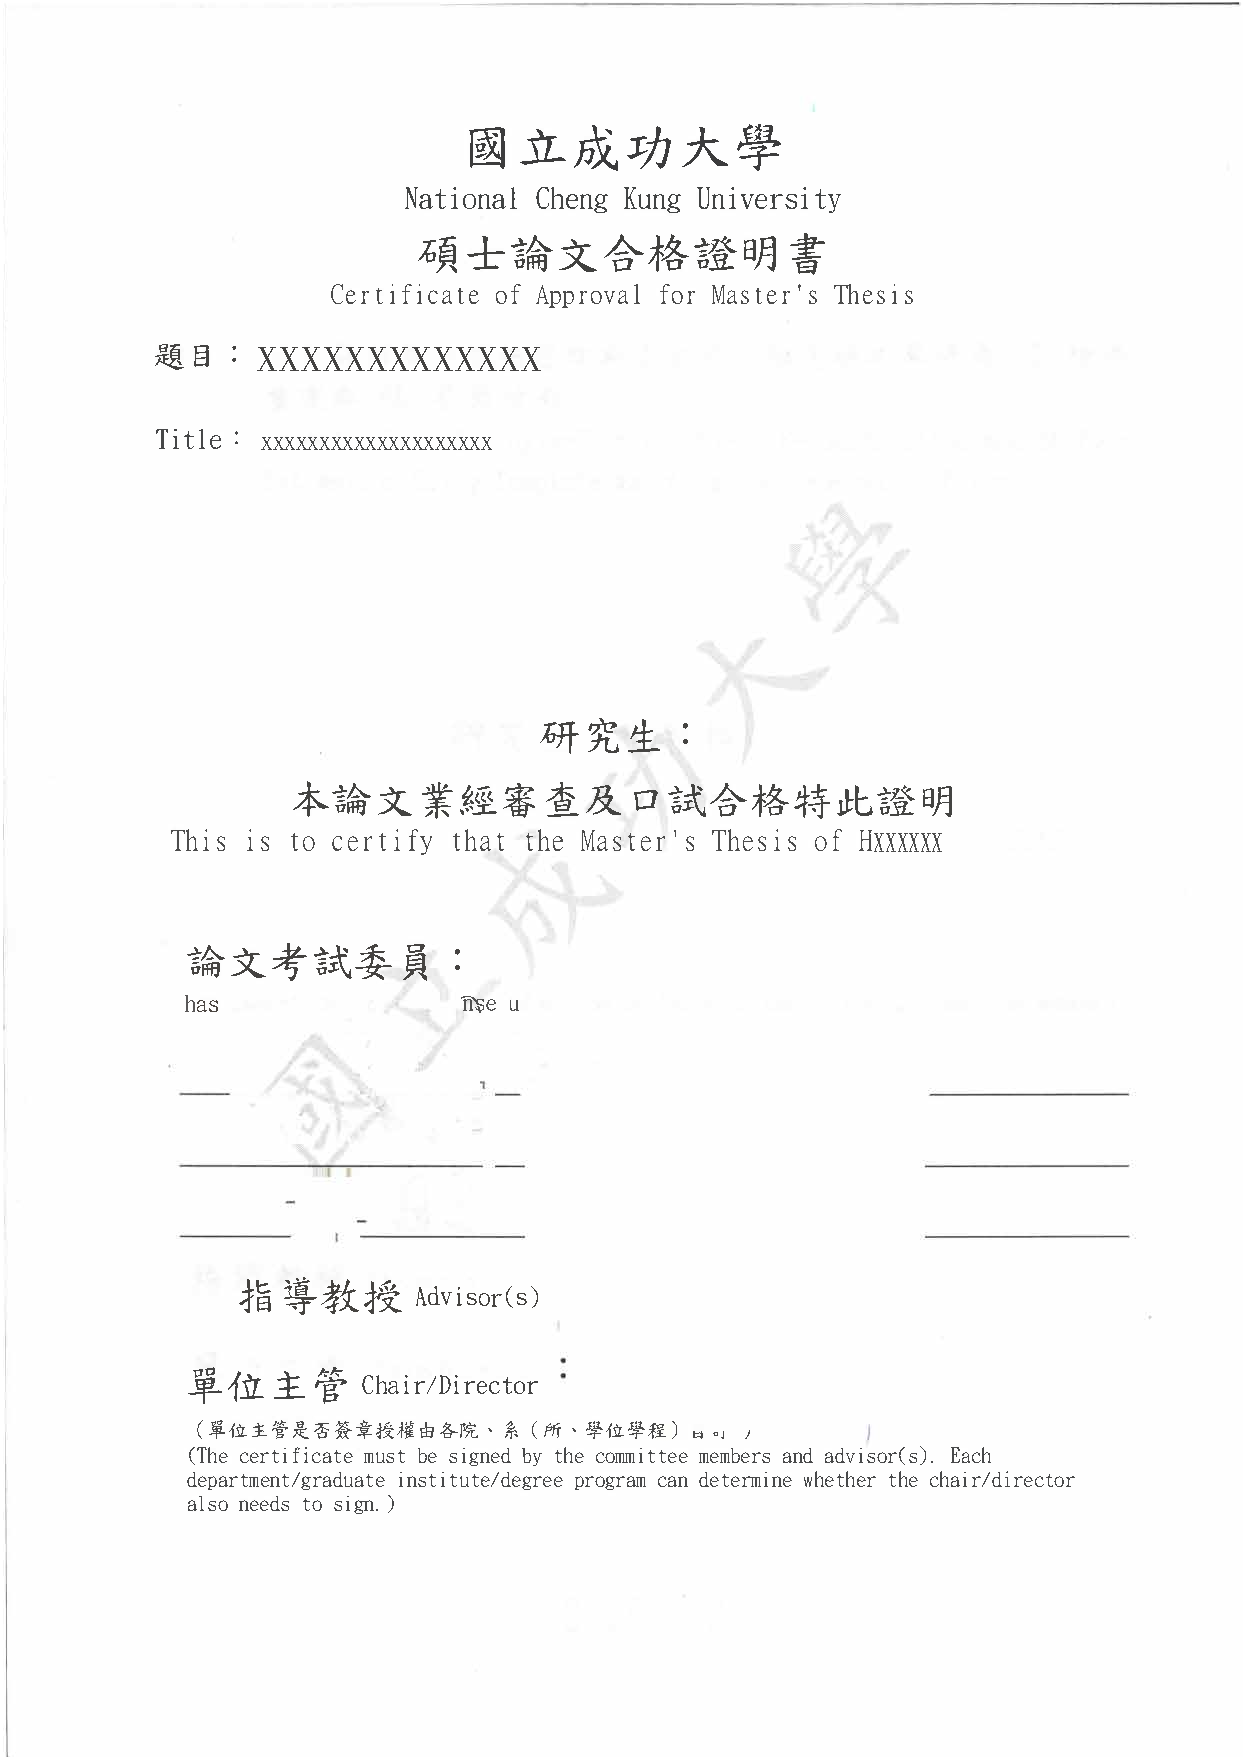
\includepdf[
    pages=1,
    pagecommand={\thispagestyle{empty}},
    fitpaper=true
]{frontpages/SCAN.pdf}




%%%%%%%%%%%%%%%%%%%%%%%%%%%%%%%
%       中文摘要
%%%%%%%%%%%%%%%%%%%%%%%%%%%%%%%

% 可以利用如下自定義的command (定義在nckuee.sty)
% ======
%\begin{zhAbstract}  %中文摘要
%\input{frontpages/front_cabstract.tex} % // 可以引入front_cabstract.tex檔案或在此編輯 // cbj
%\end{zhAbstract}

% ...等
% ======

% 在此直接定義如下
%%%%%%%%%%%%%%%%
%
%%%%%%%%%%%%%%%%%%%%%%%%%%%%%%%%%%%%%%%%%%%%%%%%%%%%%%%%%%%%%%%%
%                       中文摘要
%%%%%%%%%%%%%%%%%%%%%%%%%%%%%%%%%%%%%%%%%%%%%%%%%%%%%%%%%%%%%%%%

\newpage

% 頁碼從中文摘要開始
\setcounter{page}{1}
\pagenumbering{roman}

% 中文摘要加入目錄
\phantomsection
\addcontentsline{toc}{chapter}{\nameCabstract}


% ############################################################
% ##### 中文摘要格式開始：所有設定只作用於中文摘要 #####
% ############################################################

\begingroup

% 單行間距
\renewcommand{\baselinestretch}{1}
\selectfont

% 摘要段落不縮排
\setlength{\parindent}{0pt}

% 段落之間不額外增加空白
\setlength{\parskip}{0pt}


% ============================================================
% 中文論文題目
% 14 pt、粗體、置中
% ============================================================

\begin{center}

{\fontsize{14pt}{16pt}\selectfont
\bfseries
\zhTitle
\par}

\vspace{0.5cm}


% ============================================================
% 作者資料
% 12 pt、標準字、置中
% ============================================================

{\fontsize{12pt}{14pt}\selectfont
\normalfont

\renewcommand{\thefootnote}{\fnsymbol{footnote}}
\makebox[3.5cm][l]{\large{\authorZhName\footnote[1]{}}}\footnotetext[1]{{學生}} % 學生中文姓名
%\hfill
%
%\makebox[3cm][c]{\large{指導教授：}}
\makebox[3.5cm][l]{\large{\advisorZhName\footnote[2]{}}}\footnotetext[2]{{指導教授}} \\ %指導教授中文姓名


\zhUniv\zhDepartmentName
\par

}

\vspace{0.5cm}


% ============================================================
% 摘要標題
% 12 pt、粗體、置中
% ============================================================

{\fontsize{12pt}{14pt}\selectfont
\bfseries
摘要
\par}

\end{center}


\vspace{0.3cm}


% ============================================================
% 中文摘要內文
% 12 pt、標準字、單行間距、不縮排
% ============================================================

{\fontsize{12pt}{14pt}\selectfont
\normalfont

\input{frontpages/front_cabstract.tex}

}

\endgroup

% ############################################################
% ##### 中文摘要格式結束：後面自動恢復原論文設定 #####
% ############################################################





%%%%%%%%%%%%%%%%%%%%%%%%%%%%%%%%%%%%%%%%%%%%%%%%%%%%%%%%%%%%%%%%
%                       英文摘要
%%%%%%%%%%%%%%%%%%%%%%%%%%%%%%%%%%%%%%%%%%%%%%%%%%%%%%%%%%%%%%%%

\newpage

% 英文摘要加入目錄
\phantomsection
\addcontentsline{toc}{chapter}{\nameEabstract}


% ############################################################
% ##### 英文摘要格式開始：與中文摘要完全相同 #####
% ############################################################

\begingroup

% 單行間距
\renewcommand{\baselinestretch}{1}
\selectfont

% 摘要段落不縮排
\setlength{\parindent}{0pt}

% 段落之間不額外增加空白
\setlength{\parskip}{0pt}

% Times 字型
\rmfamily


% ============================================================
% 英文論文題目
% 14 pt、粗體、置中
% ============================================================

\begin{center}

{\fontsize{14pt}{16pt}\selectfont
\bfseries
\enTitle
\par}

\vspace{0.5cm}


% ============================================================
% 作者資料
% 12 pt、標準字、置中
% ============================================================

{\fontsize{12pt}{14pt}\selectfont
\normalfont


\renewcommand{\thefootnote}{\fnsymbol{footnote}}
\makebox[5cm][l]{\large{\authorEnName\footnote[1]{}}}\footnotetext[1]{{Student}} % 學生英文姓名
%\hfill
%
%\makebox[2cm][s]{\large{Advisor: }}
\makebox[5cm][l]{\large{\advisorEnName\footnote[2]{}}}\footnotetext[2]{{Advisor}} \\ %教授英文姓名
%

\enDepartmentName
\par

\enUniv
\par

}

\vspace{0.5cm}


% ============================================================
% ABSTRACT 標題
% 12 pt、粗體、置中
% ============================================================

{\fontsize{12pt}{14pt}\selectfont
\bfseries
ABSTRACT
\par}

\end{center}


\vspace{0.3cm}


% ============================================================
% 英文摘要內文
% 12 pt、標準字、單行間距、不縮排
% ============================================================

{\fontsize{12pt}{14pt}\selectfont
\normalfont

\input{frontpages/front_eabstract.tex}

}

\endgroup

% ############################################################
% ##### 英文摘要格式結束：後面自動恢復原論文設定 #####
% ############################################################


%%%%%%%%%%%%%%%%%%%%%%%%%%%%%%%
%       誌謝
%%%%%%%%%%%%%%%%%%%%%%%%%%%%%%%
%
% Acknowledgment
\newpage
\phantomsection % for hyperref to register this
%\addcontentsline{toc}{chapter}{\nameAcknc}

\begin{zhAckn}  %誌謝
咕咕嘎嘎

吧噗吧噗

\begin{flushright}

\end{flushright} % // 可以引入front_ackn.tex檔案或在此編輯 // cbj
\end{zhAckn}

%\chapter*{\nameAckn} %\makebox{} is fragile; need protect
%咕咕嘎嘎

吧噗吧噗

\begin{flushright}

\end{flushright} % // 可以引入my_ackn.tex檔案或在此編輯 // cbj
%%testjsjtoejiojsoijtoijos

%%%%%%%%%%%%%%%%%%%%%%%%%%%%%%%
%       目錄
%%%%%%%%%%%%%%%%%%%%%%%%%%%%%%%
%
% Table of contents
\newpage
\renewcommand{\contentsname}{\nameTocc}
%\makebox{} is fragile; need protect
\phantomsection % for hyperref to register this
\addcontentsline{toc}{chapter}{\nameTocc}
\tableofcontents

%%%%%%%%%%%%%%%%%%%%%%%%%%%%%%%
%       表目錄
%%%%%%%%%%%%%%%%%%%%%%%%%%%%%%%
%
% List of Tables
\newpage
\renewcommand{\listtablename}{\nameLotc}
%\makebox{} is fragile; need protect
\phantomsection % for hyperref to register this
\addcontentsline{toc}{chapter}{\nameLotc}
\listoftables

%%%%%%%%%%%%%%%%%%%%%%%%%%%%%%%
%       圖目錄
%%%%%%%%%%%%%%%%%%%%%%%%%%%%%%%
%
% List of Figures
\newpage
\renewcommand{\listfigurename}{\nameTofc}
%\makebox{} is fragile; need protect
\phantomsection % for hyperref to register this
\addcontentsline{toc}{chapter}{\nameTofc}
\listoffigures
%%%%%%%%%%%%%%%%%%%%%%%%%%%%%%%
%       符號說明
%%%%%%%%%%%%%%%%%%%%%%%%%%%%%%%
%
% Symbol list
% define new environment, based on standard description environment
% adapted from p.60~64, <<The LaTeX Companion>>, 1994, ISBN 0-201-54199-8

%\newcommand{\SymEntryLabel}[1]%
%  {\makebox[3cm][l]{#1}}
%%
%\newenvironment{SymEntry}
%   {\begin{list}{}%
%       {\renewcommand{\makelabel}{\SymEntryLabel}%
%        \setlength{\labelwidth}{3cm}%
%        \setlength{\leftmargin}{\labelwidth}%
%        }%
%   }%
%   {\end{list}}
%%%
%\newpage
%\chapter*{\nameSlist} %\makebox{} is fragile; need protect
%\phantomsection % for hyperref to register this
%\addcontentsline{toc}{chapter}{\nameSlistc}
%\input{frontpages/front_symbols.tex}

\newpage
\setcounter{page}{1}
\pagenumbering{arabic}

% 主要是 overleaf 免費版編譯有限制時間，針對某些不要的章節註解可以避免compile時間過長
% overleaf 編譯超時，你就多分一個檔XD



\chapter{Introduction} \label{ch:1-introduction}
\hspace{24pt}

Add your introduction here.

\section{Mathematic Symbols}
% *** mathematic symbols (use dollar sign to wrap it)***
$C_t$ example of sub
$C^t$ example of power
% more symbols in latex : https://en.wikipedia.org/wiki/Wikipedia:LaTeX_symbols

\section{Equation}
% *** example of equation ***
Below is equation~\ref{eq:example}.
\begin{eqnarray}
        C_t=\{x|x \in P \wedge D(t,x) \leq \delta \wedge A(x) > 0 \}.
        \label{eq:example}
\end{eqnarray}
% more about equation in latex :  https://en.wikibooks.org/wiki/LaTeX/Advanced_Mathematics

\section{Step lists}
\begin{description}
    \item [Step 1.] balabala
    \item [Step 2.] balabala
\end{description}

\section{Algorithm}
% *** example of algorithm ***
% require \usepackage{algorithm}
We proposed algorithm ~\ref{algorithm:example}.


\begin{algorithm}[H]
    \caption{Standard RANSAC-PnP Method Based on for Outlier Rejection}
    \label{algorithm:example}
    % \small % 縮小演算法字體，進一步節省空間
    \begin{algorithmic}[1]
         % === 在這裡加入這三行來壓縮行與行的上下間距 ===
        \setlength{\itemsep}{1pt}       % 調整每個步驟之間的垂直距離
        \setlength{\parsep}{0pt}        % 調整段落之間的距離
        \linespread{0.9}\selectfont     % 稍微壓縮文字本身的行高（可依需求改 0.85 或 0.95）
        % ===========================================
        \Require 2D--3D correspondences $\{(x_i, X_i)\}_{i=1}^{N}$,
                 camera intrinsic matrix $K$,
                 reprojection threshold $\tau$,
                 maximum iterations $M$
        \Ensure Best pose $(R,t)$ and inlier set $\mathcal{I}$

        \State $bestInliers \gets \emptyset$
        \State $bestPose \gets \emptyset$

        \For{$k = 1$ to $M$}
            \State Randomly select a minimal subset of correspondences
            \State Estimate pose $(R,t)$ using PnP
            \State $\mathcal{I} \gets \emptyset$

            \For{each correspondence $(x_i, X_i)$}
                % 將公式直接合併到 \State 中，改用 $ ... $
                \State Project $X_i$ onto the image: $\hat{x}_i = \pi(K,R,t,X_i)$
                \State Compute reprojection error: $e_i = \|x_i-\hat{x}_i\|$

                \If{$e_i < \tau$}
                    \State Add $(x_i,X_i)$ to $\mathcal{I}$
                \EndIf
            \EndFor

            \If{$|\mathcal{I}| > |bestInliers|$}
                \State $bestInliers \gets \mathcal{I}$
                \State $bestPose \gets (R,t)$
            \EndIf
        \EndFor
        \State Re-estimate $(R,t)$ using all correspondences in $bestInliers$
        \State \Return $bestPose$, $bestInliers$
    \end{algorithmic}
\end{algorithm}
% more about algorithm in latex : https://en.wikibooks.org/wiki/LaTeX/Algorithms (Typesetting using the algorithmicx package)
% http://ftp.yzu.edu.tw/CTAN/macros/latex/contrib/algorithms/algorithms.pdf

\section{Label} \label{subsec: labelName}
This is Section~\ref{subsec: labelName}.

\section{Reference}
Professor Tsai published many good papers~\cite{TsaimhPaper}.

\section{Subsection}
\subsection{one}


\section{Table}
% *** Table ***
Table~\ref{tab:example} is a 3 x 3 table.
\begin{table}[h] 
    \normalsize
    \caption{Table Example} 
    \begin{center} 
        \label{tab:example} 
        \begin{tabular}{ | l | c || r |}
            % use | to draw the vertical line
            % use \hline to draw horizontal line
            \hline
            1 & 2 & 3 \\ \hline\hline
            4 & 5 & 6 \\ \hline
            7 & 8 & 9 \\ 
            \hline
        \end{tabular} 
    \end{center} 
\end{table}
% more about table in latex :  https://en.wikibooks.org/wiki/LaTeX/Tables

\section{Figure}
% *** figure ***
Figure~\ref{fig:introduction_overview} is flowchart.


\begin{figure}[h]
    \begin{center}
        
\includegraphics[width=0.95\textwidth]{images/introduction_overview.jpg}
    \end{center}
    \caption{整體架構圖}
    \label{fig:introduction_overview}
\end{figure}

\chapter{Related Work} \label{ch:2-related-works}
% 
\hspace{24pt}
\section{Section}
\subsection{Subsection}

Add your related works here.
SAM3D\cite{sam3d2025} SAM3D\cite{sam3d2025, diffdope2023}


\chapter{Method} \label{ch:3-method}
\section{Overview}
\hspace{24pt}

哈哈哈

\revision{偷尼說修改要用紅色標記}拉拉拉


或是這樣
\revision{3.1415926535

8979323846

2643383279}

\section{你}
\subsection{決}
\subsubsection{定}

\chapter{Experimental Results} \label{ch:4-results}
\section{OOO定性分析與討論}

% \section{OOO定量分析與討論}

% 
\section{OOO更多結果}


\chapter{Conclusion} \label{ch:5-conclusion}
% \section{結論與主要貢獻 (Conclusions and Contributions)}
Add your conclusions here.

\section{研究限制 (Limitations)}
Add your conclusions here.

\section{未來研究方向 (Future Work)}
Add your conclusions here.


\input{back/back_reference.tex}

\clearpage % to make sure all CJK characters are processed
\end{CJK}  %%% ZZZ %%%
\end{document}